\chapter{Einführung}
Im Rahmen dieser Belegarbeit soll ein Ansatz entwickelt werden, um in Java oder Scala auf Clustern auf Grafikkarten zu berechnen. Es wurde sich für eine Kombination von Spark für die Kommunikation im Cluster und Rootbeer für die Grafikkartenprogrammierung entschieden.

Zuerst wird in den Kapiteln \ref{sct:montecarloalgo}-\ref{sct:spark} die benutzten Algorithmen und Bibliotheken vorgestellt, in Kapitel~\ref{sct:implementation} wird die eigene Implementierung dokumentiert und in Kapitel~\ref{sct:benchmarks} werden Benchmarks dieser Implementierung vorgestellt.

%Dabei soll die Vorgehensweise reproduzierbar dokumentiert werden, mit dem Ziel, die Programmierung auf Grafikkarten-Clustern so einfach wie möglich zu machen. Z.B. durch ein Skript. Als ersten Testfall wird ein Monte-Carlo-Algorithmus zur Berechnung von Pi implementiert, da dieser sehr rechenlastig ist. Weiterhin soll ein kommunikationslastiger Algorithmus wie z.B. Mergesort auf einem Grafikkartencluster untersucht werden.

\chapter{Rechenintensiver Testalgorithmus}
\label{sct:montecarloalgo}

\section{Monte-Carlo Algorithmen}

Monte-Carlo-Algorithmen bezeichnet Algorithmen, die mit Hilfe von (Pseudo-)Zufallszahlen versuchen das gesuchte Ergebnis statistisch zu approximieren. Dafür werden Stichproben aus statistischen Verteilungen durch z.B. physkalisch begründete Abbildungen transformiert und jene Ergebnisse statistisch ausgewertet. Diese Art von Verfahren eignet sich z.B. zur Berechnung von Integralen über zig Koordinaten, die mit üblichen Newton-Cotes-Formeln aufgrund der hohen Dimensionalität nicht praktikabel wären. Eine andere Anwendung ist die Analyse von durch kosmischer Strahlung ausgelösten Teilchenschauern mit Hilfe von Markov-Ketten\cite{metropolis1949monte}.

Monte-Carlo-Algorithmen sind als statistische Stichprobenverfahren schon länger bekannt, wurden aber erst mit dem Aufkommen der ersten Computer, z.B. dem ENIAC um 1947-1949, praktikabel\cite{metropolis1987beginning}. Der Name, nach der Spielbank ''Monte-Carlo'', wurde von N.Metropolis vorgeschlagen und hielt sich seitdem. Der Vorschlag zu dieser Art von Algorithmus kam von John von Neumann auf, als man mit dem ENIAC thermonukleare Reaktionen simulieren wollte. Aber Fermi wird nachgesagt schon Jahre zuvor statistische Stichprobenverfahren in schaflosen Nächten händisch angewandt zu haben und mit den überraschend genauen Resultaten seine Kollegen in Staunen zu versetzen.

Monte-Carlo-Verfahren sind inhärent leicht zu parallelisieren, da eine Operation, die Simulation, mehrere Tausend oder Milliarden Mal ausgeführt wird. Eine Schwierigkeit besteht jedoch darin den Pseudozufallszahlengenerator (pseudorandom number generator - PRNG) korrekt zu parallelisieren. Das heißt vor allem muss man unabhängige Startwerte finden und an die parallelen Prozesse verteilen.
 - Zeitangaben sind hierbei nicht sinnvoll. Das betrifft alle möglichen Zeitgeber in Rechnern wie z.B. .

\subsection{Berechnung von Pi}

Um Pi zu berechnen wird Pi als Integral dargestellt, da sich beschränkte Integrale durch Monte-Carlo-Verfahren approximieren lassen.
\begin{equation}
	\pi = \int \begin{cases}
					1 & |x^2+y^2| \leq 1\\
					0 & \text{sonst}
			   \end{cases}
		  \mathrm{d}x \mathrm{d}y
\end{equation}
Das heißt wir integrieren die Fläche eines Einheitskreises. Durch die Ungleichung wissen wir auch, dass nur für $x,y\in [-1,1]$ der Integrand ungleich $0$ ist.

Da es programmatisch trivialer ist Zufallszahlen aus dem Intervall $[0,1]$ anstatt $[-1,1]$ zu ziehen, wird das Integral über den Einheitskreis in ein Integral über einen Viertelkreis geändert:
\begin{equation}
	\label{eq:piint}
	\pi = 4 \int\limits_{0}^\infty \mathrm{d}x
		    \int\limits_{0}^\infty \mathrm{d}y
		    \begin{cases}1 & |x^2+y^2| \leq 1\\0 & \text{sonst} \end{cases}
\end{equation}

Das Vorgehen ist nun wie folgt
\begin{enumerate}
	\item Setze die Zählvariable \texttt{Summe} auf $0$
	\item Ziehe für $x$ und $y$ je eine gleichverteilte Zufallszahl aus dem Intervall $[0,1]$\
	\item Falls $x^2+y^2<1$, dann erhöhe \texttt{Summe} um $1$
	\item Gehe zu 2.
\end{enumerate}
Mathematisch ausgedrückt also:
\begin{equation}
	\label{eq:pimonteint}
	\mu_N = \langle f\left( \vec{x}_i \right) \rangle := \frac{1}{N} \sum_{i=1}^N f\left( \vec{x}_i \right),\;\vec{x}_i \text{ uniform zufallsverteilt aus } \Omega:=[0,1]\times[0,1]
\end{equation}
Im allgemein ist $f$ eine beliebige Funktion, aber für die Berechnung von Pi ist es die Einheitskugel in 2D, vgl.Gl.\ref{eq:piint}.

In Python kann man dies, wenn man sich auf Einkernprozessoren einschränkt, mit NumPy\cite{numpy} in nur wenigen zeilen niederschreiben:
\begin{lstlisting}[language=python]
from numpy import *
N=10000000
x=random.rand(N)
y=random.rand(N)
pi = 4.0 * sum( x*x + y*y < 1 ) / N
\end{lstlisting}\vspace{-1.5\baselineskip}

Der Vollständigkeit halber seien kurz ein paar Worte zu den Rändern verloren, das betrifft die Zufallszahlen die entweder aus einem rechtsoffenem oder geschlossenen Intervall $[0,1]$ stammen können und den Vergleich, der die Gleichheit mit einschließen kann oder nicht.

Aus der Integraltheorie ist klar, dass die Ränder ein Nullmaß haben und damit keine Rolle spielen. Aber für diskrete Verfahren könnte dies zu einer zusätzlichen systematischen Fehlerquelle führen, der Fehlerskalierverhalten möglicherweise beeinträchtigt.

Am Beispiel von nur vier Zuständen für Zufallszahlen für den rechtsoffenen Fall, also $x,y\in \lbrace 0,0.25,0.5,0.75 \rbrace$, sei dies einmal durchgedacht. Damit ergibt sich
\begin{equation}
	x^2+y^2 = \lbrace 0, 0.0625, 0.125, 0.25, 0.3125, 0.5, 0.5625, 0.625, 0.8125, 1.125 \rbrace
\end{equation}
% (Python-Skript für Kombinationen:
%    x=array([0,1,2,3])/4.
%    a,b=meshgrid(x**2,x**2)
%    unique( (a+b).ravel() )
Hier macht es aufgrund der begrenzten Anzahl an Zuständen, unter denen die $1.0$ ohnehin nicht auftritt, keinen Unterschied ob man $<$ oder $\leq$ vergleicht, man erhielte Pi zu $3.6$.
Hinzu kommt aber, dass Zustände auf den Grenzen $x=0$ und $y=0$ liegen, sodass die Grenzen vierfach gezählt werden da wir nur den Viertelkreis berechnen und mit vier multiplizieren.

Man hat also ohnehin immer einen Diskretisierungsfehler von $O\Delta x)$ wobei $\Delta x$ die Diskretisierungslänge zwischen zwei Zuständen ist. Angemerkt sei, dass dies für Gleitkommazahlen komplizierter gestaltet.

Abschließend sei angemerkt, dass Monte-Carlo-Methoden dafür gedacht sind einen praktisch unerschöpflichen Raum Stichprobenartig auszutesten, sodass Diskretisierungs- und Randfehler ohnehin als vernachlässigbar angenommen werden. Wenn man merkt, dass es zu Diskretisierungsfehler wie obig an den Rändern kommt, oder man gar die Anzahl aller möglichen Zustände an Zufallszahlen erschöpft hat und sich die Approximation damit nicht mehr verbessern kann, sollte man über ein anderes Verfahren nachdenken oder den Zufallsgenerator anpassen und z.B. mit 128-Bit statt 32-Bit betreiben. Auch die maximale Periodenlänge von Pseudozufallsgeneratoren spielt hier eine Rolle!
%
%Mit geschlossenen Grenzen hingegen wären $x,y\in\lbrace 0,\frac{1}{3},\frac{2}{3},1 \Rightarrow \rbrace 0, \frac{1}{9}, \frac{2}{9}, \frac{4}{9}, \frac{5}{9}, \frac{8}{9}, 1 \frac{10}{9}, \frac{13}{9},2 \rbrace$
% Man beachte, dass float ohnehin nur 32 Bit ist, wovon 1 bit das Vorzeichen und 8 bit der Exponent ist. Da wir uns immer nur im Intervall [0,1] befinden nutzen wir Vorzeichen und Exponent ohnehin nicht, sodass nur 23 Bit Präzision benutzt werden. Das sind also nur 2^23 \approx 10^7 erreichbare Zustände. Moderne Prozessoren können leicht 10^9 Operationen pro Sekunde rechnen, sodass einfache Fließkommagenauigkeit nicht ausreicht, da schon nach einigen Millionen Stichproben sich der relative Fehler nicht mehr verbessern, aber auch nciht mehr verschlechtern, wird. Siehe dazu Abb.\ref{fig:monteerrorfloat}

Da die Monte-Carlo-Pi-Integration einer Mittelwertbildung entspricht, vgl. Gl.\ref{eq:pimonteint}, ist die statistische Unsicherheit gegeben durch die Standardabweichung des Mittelwerts $\sigma_{\mu_N}$, welche gegeben ist als
\begin{equation}
	\sigma_{\mu_N} \frac{\sigma}{\sqrt{N}}
\end{equation}
wobei $\sigma$ die Standardabweichung der Stichprobe ist, vgl. Anhang~\ref{apx:meanerror}.
Wenn $f_i$ in einem beschränkten Intervall liegt, dann ist auch die Standardabweichung der Stichproben $f_i$ beschränkt, sodass die Standardabweichung auf den Mittelwert $\propto \frac{1}{\sqrt{N}}$ abnimmt.

\begin{figure}
	\centering
	\begin{minipage}{0.7\linewidth}
		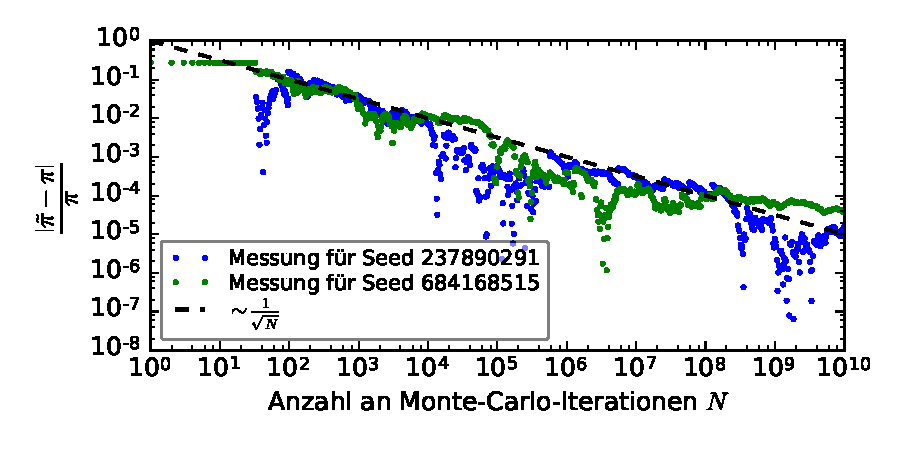
\includegraphics[width=\linewidth]{monte-carlo-pi-error-scaling}
	\end{minipage}
	\caption{captiontext}
	\label{fig:monteerrorfloat}
\end{figure}


%\subsection{Pseudozufallszahlgeneratoren}
%\section{Vergleich - Alternativen}
